\documentclass[titlepage,a4paper,12pt,thmsb]{report}

\usepackage{graphicx}
\usepackage{graphics}
\usepackage[english]{babel}
\usepackage{float,epsfig, floatflt,here}
\usepackage{amsmath}
\usepackage{a4}
\usepackage{fancyhdr}
\usepackage{makeidx}
\usepackage{hyperref}
\usepackage{moreverb}
%\usepackage{loremipsum}
\usepackage{tabularx}
\usepackage{tabulary}

\textwidth 16cm \textheight 22.5cm \selectlanguage{english}
\topmargin 0cm \headheight 0.5 cm \oddsidemargin 0cm
\evensidemargin 0cm
\renewcommand{\baselinestretch} {1.2} \setlength{\parindent}{0.0cm}
\setlength{\parskip} {0.5 cm}
%\renewcommand{\thesection}{\arabic{section}}
\renewcommand{\thechapter}{\arabic{chapter}}
\setcounter {secnumdepth}{5} \setcounter{tocdepth}{5}
\let\oldTitle\title
\renewcommand{\title}[1]{\newcommand{\myTitle}{#1}\oldTitle{#1}}
\newcommand{\leftscripts}[3]{{\vphantom{#3}}^{#1}_{#2}{#3}}

%%% Fancy Header %%%%%%%%%%%%%%%%%%%%%%%%%%%%%%%%%%%%%%%%%%%%%%%%%%%%%%%%%%%%%%%%%%
% Fancy Header Style Options
\pagestyle{fancyplain}                  % Sets fancy header and footer
%\fancyfoot{}                           % Delete current footer settings
\renewcommand{\chaptermark}[1]{         % Lower Case Chapter marker style
  \markboth{\chaptername\ \thechapter.\ #1}{}} %
\renewcommand{\sectionmark}[1]{         % Lower case Section marker style
  \markright{\thesection.\ #1}}         %
\fancyhead[LE,RO]{\thepage}             % Page number (boldface) in left on even
                                        % pages and right on odd pages
%\fancyhead[RE]{\bfseries\leftmark}     % Chapter in the right on even pages
\fancyhead[RE]{\leftmark}               % Chapter in the right on even pages
%\fancyhead[LO]{\bfseries\rightmark}    % Section in the left on odd pages
\fancyhead[LO]{\rightmark}              % Section in the left on odd pages

\renewcommand{\headrulewidth}{0.1pt}    % Width of head rule
\renewcommand\footrulewidth{0.1pt}
%\fancyfoot[CE,CO]{\myTitle}{}
\fancyfoot[CE,CO]{CS212 Intelligent Data Analysis}{}
\makeindex
%%%%%%%%%%%%%%%%%%%%%%%%%%%%%%%%%%%%%%%%%%%%%%%%%%%%%%%%%%%%%%%%%%%%%%%%%%%%%%%%%%%%%%%
%\let\oldAuthor\author
%\renewcommand{\author}[1]{\newcommand{\myAuthor}{#1}\oldAuthor{#1}}
%%%%%%%%%%%%%%%%%%%%%%%%%%%%%%%%%%%%%%%%%%%%%%%%%%%%%%%%%%%%%%%%%%%%%%%%%%%%%%%%%%%%%%%
\begin{document}
\pagenumbering{roman}
\begin{titlepage}
\thispagestyle{empty}
%\vspace*{0.7cm}
\begin{center}
%{\centering
%\large
{\LARGE \bf{ Investigating Properties of Forest Fires from a 13-Dimensional
Data Set}} \\
\vspace{2.0cm}
%\it{A project report submitted in partial fulfillment \\ for the requirements for the degree of \\ Master of IT in Business} \\
\large \bf{An Assignment Report of } \\
\large \bf{CS212\\ Intelligent Data Analysis} \\
\vspace{0.5cm}
%\sc
\large \sc{by} \\
\vspace{0.5cm}
\rm
{\large \bf {Xiangyi Yan}}\\
%{\large \bf {01010410}}
\vspace{0.5cm}
%\sc
\bf{11510706@mail.sustc.edu.cn} \\

\vspace{1cm}

{\sc{under the guidance of}} \\
\vspace{.5cm}

\hspace{.05cm} {\bf {Peter Ti\v{n}o}}\\
\hspace{.05cm} {\sc and}\\
\hspace{.05cm} {\bf {Guoji Fu}}\\
\vspace{0.5cm}
\vspace{0.5cm}
%\universityseal\ \\

\begin{figure}[h]
%\hspace{6cm}
%\vspace{5cm}
{\centering {\includegraphics[width=0.5\linewidth,angle=0]{logo/logo.png}}\par}
\end{figure}

\vskip 0.5cm

%\large{\bf Department of Mathematics \& Computing} \\
\large{\bf Department of Computer Science and Engineering} \\
\vskip 0.5cm
%\Large{\bf Indian Institute of Technology Guwahati}\\
\Large{\bf Southern University of Science and Technology}\\
\vskip 0.5cm
{\centering \sc{Shenzhen, China, June 2017}}
%} %%% this is end of centering environment
\end{center}
\pagebreak
\end{titlepage}


\chapter*{Abstract}
\addcontentsline{toc}{chapter}{\numberline{}CERTIFICATE}
The purpose of this assignment was to utilize dimension-reducing techniques such as {\bf principal component analysis (PCA)} and {\bf coordinate-projection} to explore relationships between varying attributes of {\bf forest fires}. It was found that some of these attributes didn’t correlate with the rest of the data (such as {\bf total phenols}),though when reduced enough, certain attributes were found to hold relationships.
\vspace*{0.5cm}\\
{\large \bf {Code \& Notable Files:}}
\newline{}
{\hspace*{0.7cm}{\url{https://github.com/yanxiangyi/forest_fire_pca}} }



\chapter*{Data Set Introduction}
{\large \bf {13 Dimensions}}
\begin{itemize}
\item{X - x-axis spatial coordinate within the Montesinho park map: 1 to 9}
\item{Y - y-axis spatial coordinate within the Montesinho park map: 2 to 9}
\item{month - Month of the year: 'jan' to 'dec' }
\item{day - Day of the week: 'mon' to 'sun' }
\item{FFMC - Fine fuel moisture code index from the FWI system: 18.7 to 96.20 }
\item{DMC - Duff moisture code index from the FWI system: 1.1 to 291.3 }
\item{DC - Drought code index from the FWI system: 7.9 to 860.6 }
\item{ISI - Initial spread index from the FWI system: 0.0 to 56.10 }
\item{temp - Temperature in Celsius degrees: 2.2 to 33.30 }
\item{RH - Relative humidity in \%: 15.0 to 100 }
\item{wind - Wind speed in km/h: 0.40 to 9.40 }
\item{rain - Outside rain in mm/m2 : 0.0 to 6.4 }
\item{area - The burned area of the forest (in ha): 0.00 to 1090.84 }
\end{itemize}
{\large \bf {Data Set Source:}}
\newline{}
{\hspace*{0.7cm}{\url{https://archive.ics.uci.edu/ml/datasets/Forest+Fires}} }
\newline{}
\vspace{0.5cm}


%\addcontentsline{toc}{chapter}{\numberline{}Abstract}

\addcontentsline{toc}{chapter}{\numberline{}Executive Summary}

%\chapter*{Preface}
%\addcontentsline{toc}{chapter}{\numberline{}Preface}
%{\bf ``Problems worthy of attack prove their worth by hitting back"}


%%-------------------------- Table of contents ---------------------------------%%
%\newpage
%%
%\centerline{{\bf {\large CONTENTS}}}
%%
%\tableofcontents{}
\newpage
\addcontentsline{toc}{chapter}{\numberline{}Table of Contents}
%\tableofcontents
%\makeindex
\newpage

\pagenumbering{arabic}

\chapter*{Preprocessing}

\section*{Replacement}

The {\bf month} and {\bf day} dimensions contain text elements. The first step of data preprocessing is to replace text elements with corresponding integers.

\section*{Normalization}

It's important to shift every attributes of the data to be centered:
$$\mathop{\mathbb{E}[X_i] = 0, i = 1,2,...d.}$$It's also important to scale the density of every attributes of the data so the standard deviation (or variance) need to be rescaled: $$\mathop{\mathbb{Var}[X_i] = 1, i = 1,2,...d.}$$Now every attribute is standardized to $\mathop{\frac{X_i - \mu}{\sigma}}$.

\section*{Drop Special Features}

After viewing the whole {\bf rain} attribute, I find 99.6\% (515/517) forest fires happened with no rain. Which is to say, only in 2 of 517 cases, forest fires happened while raining. We need to observe this feature independently, instead of using data analysis methods such as PCA or SOM. Therefore, the {\bf rain} attribute is considered as a special feature and is decided to be dropped.



\chapter*{Research Questions}

For my project, I tried to focus on the following two research questions:
\newline{}
\newline{}
{How does the rest of the dimensions influence:}

\begin{itemize}
\item{How does the area of the forest fires influenced by all the forest fires index?}
\item{Does the initial spread index of the forest fires influenced by any other features?}
\end{itemize}

\chapter{Area}
\section{Labelling}

According to {\bf \href{https://en.wikipedia.org/wiki/McArthur_Forest_Fire_Danger_Index}{McArthur Forest Fire Danger Index}}, forest fires can be labelled by area as:

\begin{center}
\begin{figure}[h]
{\centering {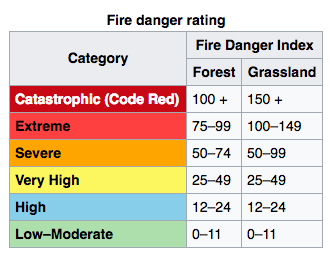
\includegraphics[width=0.6\linewidth,angle=0]{logo/category.png}}\par}
\end{figure}
{\centering{\bf{Figure 1.1.1: Fire danger rating}}}
\end{center}



\newpage

\subsection{Labelling Strategy 1}

For sake of lacking data, forest fires are labelled as three following classes (in ha):

\begin{itemize}
\item{Class 1: No Fire: 0.}
\item{Class 2: Low-Moderate: (0, 11].}
\item{Class 3: High-Catastrophic: (11, $\infty$)}
\end{itemize}

The final labelling result is:

\begin{itemize}
\item{Class 1: 247 cases.}
\item{Class 2: 183 cases.}
\item{Class 3: 87 cases.}
\end{itemize}

\begin{center}
\begin{figure}[h]
{\centering {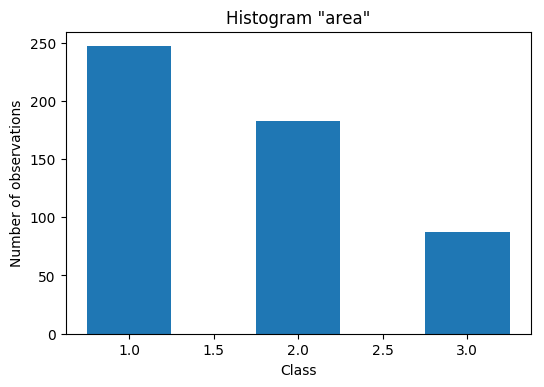
\includegraphics[width=0.7\linewidth,angle=0]{logo/Label.png}}\par}
\end{figure}
{\centering{\bf{Figure 1.1.2: Histogram of area (Labelling Strategy 1)}}}
\end{center}

\newpage

\subsection{Labelling Strategy 2}

Labelling strategy 2 aims to soften the restriction of the former one. I just put class 2 and class 3 together, which means there are only 2 classes:

\begin{itemize}
\item{Class 1: No Fire: 0.}
\item{Class 2: On fire: (0, $\infty$)}
\end{itemize}

The final labelling result is:

\begin{itemize}
\item{Class 1: 247 cases.}
\item{Class 2: 270 cases.}
\end{itemize}

\begin{center}
\begin{figure}[h]
{\centering {\includegraphics[width=0.7\linewidth,angle=0]{logo/Label2.png}}\par}
\end{figure}
{\centering{\bf{Figure 1.1.3: Histogram of area (Labeling Strategy 2)}}}
\end{center}

\newpage

\section{Straightforward Co-ordinate Projections}

In this section, let's just simply straightforward project the standardized data on a 2 dimensional plain. In {\bf{Figure 1.2.1}}, the standardized data was projected on the {\bf{FFMC}} and {\bf{wind}} plain. In {\bf{Figure 1.2.2}}, the standardized data was projected on the {\bf{FFMC}} and {\bf{DMC}} plain.

It's obviously not a good idea to do so, because we lost lots of information of the dropped dimensions. There's no apparent relationship that can be found in the following two figures.

\begin{figure}
{\centering {\includegraphics[width=0.7\linewidth,angle=0]{logo/FFMC1.png}}\par}
\end{figure}
\begin{center}


{\bf{Figure 1.2.1: Projection on FFMC and wind}}


\newpage


\begin{figure}
{\centering {\includegraphics[width=0.7\linewidth,angle=0]{logo/FFMC1_1.png}}\par}
\end{figure}

{\bf{Figure 1.2.2: Projection on FFMC and DMC}}
\end{center}

\newpage

\section{Visualization}

\subsection{Principal Component Analysis}



After normalization, the co-variance of matrix $\mathcall{X}$ can be estimated as:
$$\mathop{\mathbb{Cov}[X]} \approx \widehat{\mathop{\mathbb{Cov}[X]}} = \frac{1}{N} X X^T $$

In ${\mathop{\mathbb{Cov}[X]}}$, most of the non-diagonal elements are positive numbers, so most of them are positive related, which means most of dimensions move together in the same directions.

After ${\mathop{\mathbb{Cov}[X]}}$ calculated, \code{linalg.eig()} function in \code{numpy} was called to generate the eigenvalues, eigenvectors of the co-variance matrix.

After SVD decomposition, $\widetilde{\mathop{\mathbb{Cov}[X]}}$ can be calculated as a matrix whose diagonal elements are exactly the eigenvalues of ${\mathop{\mathbb{Cov}[X]}}$.

Before results from PCA were projected, I plotted the eigenvalue spectrum and cumulative eigenvalue plot to see how much can the first two principal components be used to represent the original relationship after the PCA projection.

The result is that the sum of first two largest eigenvalues is {\bf{0.44034744}} and the sum of first three largest eigenvalues is {\bf{0.57060657}}, which is not very ideal to project the data on a 2-dimensional or 3-dimensional plot, because we will lose about {\bf{56\%}} and {\bf{43\%}} variance of the original data, which will definitely influence the properties of the original data.

That's why in {\bf{Figure 1.7}} and {\bf{Figure 1.8}} the plot is a little bit messy. In principle component analysis, there are 11 dimensions used (without {\bf{area}} being results and {\bf{rain}} dropped).

\newpage

\begin{center}
\begin{figure}[h]
{\centering {\includegraphics[width=0.7\linewidth,angle=0]{logo/eigenvalue1.png}}\par}
\end{figure}
{\centering{\bf{Figure 1.3.1: Eigenvalues of co-variance matrix}}}
\end{center}

\begin{center}
\begin{figure}[h]
{\centering {\includegraphics[width=0.7\linewidth,angle=0]{logo/cumulative1.png}}\par}
\end{figure}
{\centering{\bf{Figure 1.3.2: Cumulative eigenvalues of co-variance matrix}}}
\end{center}

\newpage

In the following table, I list the value of the first 2 eigenvectors of ${\mathop{\mathbb{Cov}[X]}}$. The first column here shows coefficients of linear combination that defines principal component #1, and the second column shows coefficients for principal component #2. In the new axis, the new coordinates of the data are linear combination of the original coordinates and the coefficients are exactly the values in the table.

If the value is positive, then a higher score on that variable is associated with a higher score on the component, if the value is negative, then a higher score implies a lower score on the component.

In new axis #1, {\bf{CD}} index is the most important part because the coefficient is {\bf{0.46574435}}, because the value is the largest. Similarly, {\bf{Y}} is the most important part of new axis #2.

Also, in the following table, we can find that {\bf{day}} is the most useless features, because the values of {\bf{day}} for principle component #1 and principle component #2 are {\bf{0.00153541}} and {\bf{0.0034352}}. These values are too low to influence the projection. Therefore, {\bf{day}} is the most useless dimension of all 11 dimensions.


\begin{center}
{\centering{\begin{tabular}{ |l|l|l|l| }
  \hline
  \multicolumn{4}{|c|}{Top 2 largest eigenvalues and eigenvectors} \\
  \hline
  \multicolumn{2}{|c|}{1st largest: 3.29706752} &
  \multicolumn{2}{|c|}{2nd largest: 1.53738519} \\
  \hline
  Dimensions & Values & Dimensions & Values\\
  \hline
  DC & 0.46574435 & Y & -0.6927839\\
  temp & 0.42160692 & X & -0.69267032\\
  month & 0.41058638 & RH & -0.12190801\\
  DMC & 0.40663441 & DMC & -0.11283833\\
  FFMC & 0.3602159 & ISI & -0.09167051\\
  ISI & 0.29445686 & FFMC & -0.05470367\\
  RH & -0.1802439 & temp & -0.02405163\\
  wind & -0.11291306 & DC & -0.01721328\\
  X & -0.07257493 & month & -0.01517577\\
  Y & -0.06655858 & wind & 0.01230403\\
  day & 0.00153541 & day & 0.0034352\\
  \hline
\end{tabular}}}

{\centering{\bf{Table 1.3.1: Top two eigenvectors}}}
\end{center}

\newpage


\begin{center}
\begin{figure}[h]
{\centering {\includegraphics[width=0.7\linewidth,angle=0]{logo/pca1.png}}\par}
\end{figure}
{\centering{\bf{Figure 1.3.3: 2D PCA projection of area }}}
\end{center}


\begin{center}
\begin{figure}[h]
{\centering {\includegraphics[width=0.7\linewidth,angle=0]{logo/pca3d.png}}\par}
\end{figure}
{\centering{\bf{Figure 1.3.4: 3D PCA projection of area }}}
\end{center}

\newpage

\subsection{Self-organizing Map}

First, I just use SOM to fit the 11 dimensional data straightforwardly.

Obviously, plotting this is going to fool myself, because the 2D fishing net is very possible to bend a lot to fit 11D data set. The SOM would be like totally a mess.

After checking out the normal vectors of the grids in the dark center area, I confirmed my thought was right. Most of the cosine value of the normal vectors are negative values or very small values, which means that the angle between each grid is pretty large and the fishing net really curves a lot.

It's worth to mention that in this and the following SOMs, the darker the background color is, the more the "hole" of the fishing net contracts.



\begin{center}
\begin{figure}[h]
{\centering {\includegraphics[width=0.7\linewidth,angle=0]{logo/som1.png}}\par}
\end{figure}
{\centering{\bf{Figure 1.3.5: Direct SOM of 11 Dimensional data }}}
\end{center}

\newpage

Next, I used PCA to make the data reduce to 3 dimensions and used label strategy 2.

\begin{center}
\begin{figure}[h]
{\centering {\includegraphics[width=0.7\linewidth,angle=0]{logo/pca2l.png}}\par}
\end{figure}
{\centering{\bf{Figure 1.3.6: 3D PCA projection of area}}}
\end{center}

\begin{center}
\begin{figure}[h]
{\centering {\includegraphics[width=0.7\linewidth,angle=0]{logo/som3.png}}\par}
\end{figure}
{\centering{\bf{Figure 1.3.7: SOM of 3D PCA data }}}
\end{center}

We can find that the SOM is tightly contracted on the edges, and a little bit loose in the center area.

\newpage

Next, I firstly used PCA to make the data reduce to 3 dimensions and then did a 3-means clustering. After that, I plot a SOM for this 3D data.

\begin{center}
\begin{figure}[h]
{\centering {\includegraphics[width=0.7\linewidth,angle=0]{logo/cluster3.png}}\par}
\end{figure}
{\centering{\bf{Figure 1.3.8: 3D Clustering of area}}}
\end{center}

\begin{center}
\begin{figure}[h]
{\centering {\includegraphics[width=0.7\linewidth,angle=0]{logo/som2.png}}\par}
\end{figure}
{\centering{\bf{Figure 1.3.9: SOM of 3D clustering data }}}
\end{center}

We can find that the SOM is tightly contracted on the edges, and a little bit loose in the center area.


\newpage

\subsection{Comparing PCA and SOM}

After doing the above manipulation of the data, my conclusion is that:

\begin{itemize}
\item{If the data is in a high dimension, don't use SOM. Because that will definitely fool yourself. And in this condition, PCA helps a lot to visualize the data.}
\item{Try to combine these 2 techniques: do PCA first to reduce the dimension to an acceptable space(dimension) and then apply SOM to make the result of PCA easier to understand.}
\end{itemize}

\newpage

\section{Clustering}
\subsection{Clustering After PCA}

After visualization in top 3 principle components axis, we can obviously find that the data has about 2 clusters.

When I plotted the quantization error figure, the knee point is at K = 2, which means there should be 2 clusters and this can prove our former visual guess.


\begin{center}
\begin{figure}[h]
{\centering {\includegraphics[width=0.7\linewidth,angle=0]{logo/knee.png}}\par}
\end{figure}
{\centering{\bf{Figure 1.4.1: Quantization Error }}}
\end{center}

\newpage

\begin{center}
\begin{figure}[h]
{\centering {\includegraphics[width=0.7\linewidth,angle=0]{logo/cluster1_.png}}\par}
\end{figure}
{\centering{\bf{Figure 1.4.2: 1-Means Clustering }}}
\end{center}



\begin{center}
\begin{figure}[h]
{\centering {\includegraphics[width=0.7\linewidth,angle=0]{logo/cluster2_.png}}\par}
\end{figure}
{\centering{\bf{Figure 1.4.3: 2-Means Clustering }}}
\end{center}
\newpage

\begin{center}
\begin{figure}[h]
{\centering {\includegraphics[width=0.7\linewidth,angle=0]{logo/cluster3_.png}}\par}
\end{figure}
{\centering{\bf{Figure 1.4.4: 3-Means Clustering }}}
\end{center}


\begin{center}
\begin{figure}[h]
{\centering {\includegraphics[width=0.7\linewidth,angle=0]{logo/cluster4_.png}}\par}
\end{figure}
{\centering{\bf{Figure 1.4.5: 4-Means Clustering }}}
\end{center}

\newpage


\begin{center}
\begin{figure}[h]
{\centering {\includegraphics[width=0.7\linewidth,angle=0]{logo/cluster5_.png}}\par}
\end{figure}
{\centering{\bf{Figure 1.4.6: 5-Means Clustering }}}
\end{center}

\begin{center}
\begin{figure}[h]
{\centering {\includegraphics[width=0.7\linewidth,angle=0]{logo/cluster6_.png}}\par}
\end{figure}
{\centering{\bf{Figure 1.4.7: 6-Means Clustering }}}
\end{center}


\newpage

\subsection{Clustering before PCA}
Unlike the former subsection, we can't visually know how many cluster there in high dimensional space.

Therefore, we can only know from the quantization error figure, in which the knee point is also at K = 2, which means it's more possible that there are 2 clusters in the 11 dimensional space.



\begin{center}
\begin{figure}[h]
{\centering {\includegraphics[width=0.7\linewidth,angle=0]{logo/knee_.png}}\par}
\end{figure}
{\centering{\bf{Figure 1.4.8: Quantization Error}}}
\end{center}

\newpage

\begin{center}
\begin{figure}[h]
{\centering {\includegraphics[width=0.7\linewidth,angle=0]{logo/cluster1.png}}\par}
\end{figure}
{\centering{\bf{Figure 1.4.9: 1-Means Clustering }}}
\end{center}



\begin{center}
\begin{figure}[h]
{\centering {\includegraphics[width=0.7\linewidth,angle=0]{logo/cluster2.png}}\par}
\end{figure}
{\centering{\bf{Figure 1.4.10: 2-Means Clustering }}}
\end{center}
\newpage

\begin{center}
\begin{figure}[h]
{\centering {\includegraphics[width=0.7\linewidth,angle=0]{logo/cluster3.png}}\par}
\end{figure}
{\centering{\bf{Figure 1.4.11: 3-Means Clustering }}}
\end{center}


\begin{center}
\begin{figure}[h]
{\centering {\includegraphics[width=0.7\linewidth,angle=0]{logo/cluster4.png}}\par}
\end{figure}
{\centering{\bf{Figure 1.4.12: 4-Means Clustering }}}
\end{center}

\newpage


\begin{center}
\begin{figure}[h]
{\centering {\includegraphics[width=0.7\linewidth,angle=0]{logo/cluster5.png}}\par}
\end{figure}
{\centering{\bf{Figure 1.4.13: 5-Means Clustering }}}
\end{center}

\begin{center}
\begin{figure}[h]
{\centering {\includegraphics[width=0.7\linewidth,angle=0]{logo/cluster6.png}}\par}
\end{figure}
{\centering{\bf{Figure 1.4.14: 6-Means Clustering }}}
\end{center}

\newpage

\subsection{Comparing the sequence of PCA}

Comparing {\bf{Section 1.4.1}} and {\bf{Section 1.4.2}}:

The knee point is not so obvious (the angle is not that sharp) in {\bf{Figure 1.4.8}} like the one in {\bf{Figure 1.4.1}}, which means that clustering in 11 dimensional space is vaguer than the one in the former 3 dimension.

So the my conclusion is that K-means clustering may not be a good way to analysis this data set.




\newpage




\chapter{Initial Spread Index}
\section{Labelling}

According to {\bf \href{https://en.wikipedia.org/wiki/McArthur_Forest_Fire_Danger_Index}{McArthur Forest Fire Danger Index}}, forest fires can be labelled by area as:

\begin{center}
    \begin{figure}[h]
        {\centering {\includegraphics[width=0.7\linewidth,angle=0]{logo/labelling2.png}}\par}
        {\bf{Figure 2.1.1: Labelling Strategy }}
    \end{figure}
\end{center}


\newpage

For sake of lack of data, I label forest fires with three following classes (in ha):

\begin{itemize}
\item{Class 1: Low ISI: (0, 7]}
\item{Class 2: Moderate ISI: (7, 10]}
\item{Class 3: High ISI: (10, $\infty$)}
\end{itemize}

The final labelling result is:

\begin{itemize}
\item{Class 1: 145 cases.}
\item{Class 2: 217 cases.}
\item{Class 3: 155 cases.}
\end{itemize}

\begin{center}
\begin{figure}[h]
{\centering {\includegraphics[width=0.7\linewidth,angle=0]{logo/hist2.png}}\par}
{\bf{Figure 2.1.2: Histogram of ISI }}
\end{figure}
\end{center}

\newpage

\section{Straightforward Co-ordinate Projections}

In this section, let's just simply straightforward project the standardized data on a 2 dimensional plain. In {\bf{Figure 2.2.1}}, the standardized data was projected on the {\bf{FFMC}} and {\bf{wind}} plain.

From {\bf{Figure 2.2.1}}, we can approximately find the lower FFMC is, the lower the ISI is, which makes great sense because the more fine fuel in the air, the faster the forest fire can spread.




\begin{center}
    \begin{figure}
        {\centering {\includegraphics[width=0.7\linewidth,angle=0]{logo/FFMC2.png}}\par}
    \end{figure}
    {\bf{Figure 2.2.1: Projection on FFMC and wind}}
\end{center}

\newpage

\begin{center}
    \begin{figure}
        {\centering {\includegraphics[width=0.7\linewidth,angle=0]{logo/Y.png}}\par}
    \end{figure}
    {\bf{Figure 2.2.2: Projection on Y and temp}}
\end{center}

\newpage

\section{Visualization}

\subsection{Principal Component Analysis}

Like what I did in {\bf{Section 1.3}}, I used the same technique to complete this part.The result is that the sum of first two largest eigenvalues is {\bf{0.46279004}} and the sum of first three largest eigenvalues is {\bf{0.5997552}}, which is also not very ideal to project the data on a 2-dimensional or 3-dimensional plot. And that's why in {\bf{Figure 2.3.1}} and {\bf{Figure 2.3.2}} the plot is a little bit messy. In principle component analysis, there are 11 dimensions used (without {\bf{ISI}} and {\bf{area}} being results and {\bf{rain}} dropped).

Dimension {\bf{Y}} is the most important dimension, because in new axis #1 and #2, the value of {\bf{Y}} is {\bf{-0.68206234}} and {\bf{-0.68659901}}. Dimension {\bf{temp}} is the 2nd most important dimension, because in new axis #1 and #2, the value of {\bf{temp}} is {\bf{0.62039458}} and {\bf{0.64185592}}.

Initial spread speed of forest fires can be mostly affected by {\bf{Y}} and {\bf{temp}}, maybe because if the latitude is low (the coefficient is negative), it will be very hot and there will be more rotten plants and woods that can be ignited quickly, and that will accelerate the initial spread speed. When I looked back to {\bf{Figure 2.2.2}}, the figure proved my thought was right.



\begin{center}
{\centering{\begin{tabular}{ |l|l|l|l| }
  \hline
  \multicolumn{4}{|c|}{Top 2 largest eigenvalues and eigenvectors} \\
  \hline
  \multicolumn{2}{|c|}{1st largest: 3.29706752} &
  \multicolumn{2}{|c|}{2nd largest: 1.53738519} \\
  \hline
  Dimensions & Values & Dimensions & Values\\
  \hline
  Y & -0.68206234 & Y & -0.68659901\\
  temp & 0.62039458 & temp & 0.64185592\\
  DC & 0.3283881 & DC & -0.28270006\\
  month & 0.13147483 & month & 0.14181775\\
  X & -0.08656373 & X & -0.07572487\\
  RH & -0.0844196 & wind & -0.05896374\\
  FFMC & -0.07047972 & DMC & -0.05662879\\
  DMC & -0.07024343 & RH & 0.05064913\\
  wind & 0.01595388 & day & 0.03558612\\
  day & 0.00107296 & FFMC & 0.01793505\\
  \hline
\end{tabular}}}

{\centering{\bf{Table 2.3.1: Top two eigenvectors}}}
\end{center}

\newpage

\begin{center}
\begin{figure}[h]
{\centering {\includegraphics[width=0.7\linewidth,angle=0]{logo/eigenvalue2.png}}\par}
\end{figure}
{\centering{\bf{Figure 2.3.1: Eigenvalues of co-variance matrix}}}
\end{center}

\begin{center}
\begin{figure}[h]
{\centering {\includegraphics[width=0.7\linewidth,angle=0]{logo/cumulative2.png}}\par}
\end{figure}
{\centering{\bf{Figure 2.3.2: Cumulative eigenvalues of co-variance matrix}}}
\end{center}

\newpage

\begin{center}
\begin{figure}[h]
{\centering {\includegraphics[width=0.7\linewidth,angle=0]{logo/pca2.png}}\par}
\end{figure}
{\centering{\bf{Figure 2.3.3: 2D PCA projection of ISI }}}
\end{center}

\begin{center}
\begin{figure}[h]
{\centering {\includegraphics[width=0.7\linewidth,angle=0]{logo/pca3d.png}}\par}
\end{figure}
{\centering{\bf{Figure 2.3.4: 3D PCA projection of ISI }}}
\end{center}

\newpage

\section{Conclusion}

As discussed above, ISI is most influenced by {\bf{Y}} coordinates and {\bf{temp}}, although the 2D and 3D PCA projection is not that obvious to observe.

Due to the limitation of working time and similarity of works, SOM and clustering were only written in {\bf{Chapter 1}} (In {\bf{Chapter 1}}, all requirements are covered!).

In future, I will continue working on the this chapter!

Thanks, Peter! You are really a perfect teacher!

We're looking forward to your next visit!

\bibliographystyle{plain}
\bibliography{cimne}
\end{document}
